% DRAFT of the network part (27 Nov 2026). Not included in main.tex or body.tex: edit here, then paste each block where its comment says.
% Numbers: 1 Jan 2024 split, 14 themes (themes_full_v3.json). Sources: data/processed/topic_cooccurrence_network.json, topic_network_centrality.json,
% topic_link_communities.json, topic_network_lift_periods.json, topic_network_cohorts.json, reply_network_stats.json (whole subreddit),
% reply_network_stats_comments_only.json, reply_findings.json. Citation keys are in references.bib. The commenter network is not used (27 Nov).
% Length: about one page of text plus one full-width figure.

% =====================================================================================================================
% (1) RESULTS -- paste after the topic results (replaces "\subsection*{TODO}" in body.tex)
% =====================================================================================================================

\subsection*{Politics grew beside the original debate, not into it}
We built a topic network by linking two of the 123 topics when more people wrote in both than expected by chance (Methods). Of 7{,}503 possible topic pairs, 299 pass. Thirty-two niche topics, such as MSG, hummus and salt, have no link, two small groups are linked only among themselves, and the rest form one connected network (Fig.~\ref{fig:topicnet}).

The saturated-fat topic is the hub of the network: it links to 34 other topics and ranks first on degree, betweenness, closeness and eigenvector centrality. The network splits into clear communities (modularity 0.43, stable across 20 runs, AMI 0.80). The largest is about diet, weight and saturated fat; another joins omega-6 biochemistry with animal foods such as pork and raw milk; and the politics topics sit with distrust of industry and media and with arguments about studies and evidence.

None of the five politics topics links to a topic outside its community. Before 2024 they were written by the same people no more often than chance (lift 0.93, 95\% interval 0.52--1.37); from 2024 they were written together 1.57 times as often (1.39--1.76), while the rest of the network kept its shape (Fig.~\ref{fig:topiclift}).

\begin{figure}[t]\centering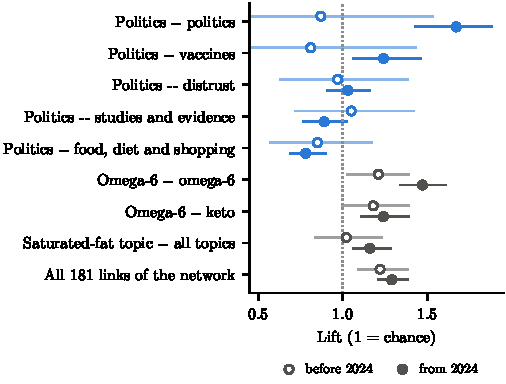
\includegraphics[width=\linewidth]{figures/topic_lift_periods.pdf}
\caption{\textbf{Co-writing before and from 2024.} Lift (people who wrote in both topics divided by the number expected by chance, summed over the topic pairs of each row) before 2024 (open, 2{,}425 people) and from 2024 (filled, 8{,}178 people), each against its own curveball null; bars are 95\% bootstrap intervals; 1 = chance. Politics changes most: its topics become a bundle and move away from food; the omega-6 topics are written together a little more, and the hub and the network as a whole stay the same.}
\label{fig:topiclift}\end{figure}

\begin{figure*}[t]\centering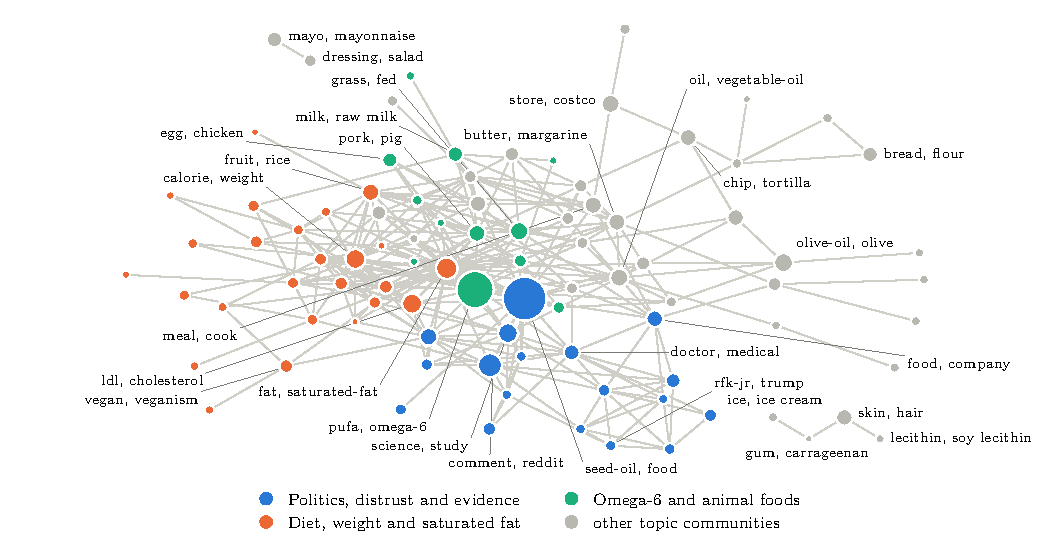
\includegraphics[width=\textwidth]{figures/topic_network_main.pdf}
\caption{\textbf{Which topics the same people write about.} Each circle is one of the 85 BERTopic topics in the main connected network (area: number of documents); a link means more people wrote in both topics than in all 500 randomisations that keep every person's number of topics and every topic's number of people (curveball null, Benjamini--Hochberg $q=0.01$). Colours: the three largest Louvain communities; grey: smaller communities, including two small groups not linked to the rest. The saturated-fat topic is the hub; the politics topics (bottom right) link only to each other and to distrust, evidence and subreddit talk. 32 topics without a significant link are not shown.}
\label{fig:topicnet}\end{figure*}

\subsection*{Old and new members took up politics alike and did not split apart}
Newcomers, accounts that first posted or commented in 2024 or later, made up 90\% of the people who wrote from 2024. Yet newcomers and long-time members alike wrote the politics topics together more often than chance (lift 1.67 and 1.44). Among the 815 long-time members who wrote before and from 2024, the politics topics went from chance (0.89) to 1.51 times chance. In the reply network of the whole r/StopEatingSeedOils subreddit (Methods), replies are strongly mutual (reciprocity 0.40, against 0.03 in a randomised network), and from 2024 long-time members and newcomers replied to each other about as often as their activity predicts (lift 0.95).

% =====================================================================================================================
% (2) METHODS -- paste into \matmethods{...} in body.tex (replaces "\textbf{Networks.} TODO." and the network part of "Checks")
% =====================================================================================================================

\textbf{Topic network.} For the 9{,}912 accounts that wrote documents in at least two topics, we built a binary person--topic matrix (1 if the person wrote at least one document in the topic). The observed weight of a topic pair is the number of people who wrote in both. The null model is the curveball algorithm \cite{strona2014curveball}, which randomises the matrix while keeping every row and column total; we drew 500 samples (burn-in of ten swaps per person, two per person between samples). A pair is linked if it is above all 500 null values and significant after Benjamini--Hochberg correction \cite{benjamini1995fdr} at $q=0.01$ on the z-score; the link weight is the ratio of observed to expected. Communities: Louvain \cite{blondel2008louvain}, best modularity of 20 seeds. Centrality: degree, betweenness and closeness with distance 1/weight, eigenvector centrality with the weights, and the participation coefficient \cite{guimera2005cartography}. Before and after 2024 we kept the all-years network as the structure and measured co-writing in each period with all people active in it (2{,}425 before 2024, 8{,}178 from 2024, each with documents in two or more topics in that period): the lift of a set of topic pairs is the number of people who wrote in both topics, summed over the pairs, divided by the number expected from that period's own curveball null (500 samples); 95\% intervals come from 400 bootstrap resamples of the period's people. Comparing lifts instead of counting significant links avoids mistaking the smaller sample before 2024 for weaker ties. \\
\textbf{Newcomers.} An account whose first post or comment in r/StopEatingSeedOils is on or after 1 January 2024; all other accounts are long-time members. The same definition is used for the topic network and the reply network. For the cohort comparison, the topic-network lifts were computed separately from each group's documents from 2024 (6{,}962 newcomers and 1{,}216 long-time members with documents in two or more topics), each against its own curveball null, and for a panel of the 815 long-time members with documents in two or more topics in both periods. \\
\textbf{Reply network.} A directed link from A to B for each comment by A that replies to a post or comment by B, weighted by the number of such replies; all accounts and the whole history, with bots, deleted accounts and self-replies removed (26{,}752 accounts, 179{,}665 links). Reciprocity is compared with a null that shuffles reply targets while keeping every account's number of replies sent and received. Mixing between newcomers and long-time members uses replies from 2024: the share of replies from one group to the other divided by the product of the first group's share of replies sent and the second group's share of replies received (1 = as expected from activity alone).

% =====================================================================================================================
% (3) DISCUSSION -- optional sentence(s) to add to the Discussion in body.tex
% =====================================================================================================================

% The networks answer the question the topic model leaves open. The political wave stayed a separate bundle of topics, not wired into the
% debate about fats, and it was taken up by long-time members as well as newcomers; in conversation the two groups kept answering each other
% about as often as chance predicts, even as politics faded after 2024. What the networks miss: they count shared topics and replies, not agreement; topics need comments of
% 15+ words; replies are counted between accounts, not by thread.
